This section describes how to use CombLayer from a user's (i.e. non-developer) point of view.
In this guide, it is assumed that the user has no C++ or coding experience.

The guide is focused on the ESS model, which can be generated by running. 
\begin{bash}
  ./ess -r modelOut
\end{bash}
This command produces the \mcnp input file {\tt modelOut1.x} as well as two other files: {\tt ObjectRegister.txt} and {\tt Renumber.txt}.

The single flag {\tt -r} is optional for MCNP6 as it causes the objects and surfaces in MCNP to be renumbered sequentially and
to fit within the 100,000 object/surface limits of MCNPX.

\subsection{Variables}
In the beginning of the input file there is a commented list of variables which define the geometry:

\begin{deck}
 c ----------------------------------------------
 c --------------- VARIABLE CARDS ---------------
 c ----------------------------------------------
 c ABunkerFloorDepth 120
 c ABunkerFloorThick 100
 c ABunkerLeftAngle 0
 c ABunkerLeftPhase -65
 c ABunkerNLayers 1
 ...
\end{deck}

The variable name consists of the component name and its corresponding parameter. For instance,
the first variable {\tt ABunkerFloorDepth} in the list above sets the floor depth of the component called {\tt ABunker}.

Only variables that have needed to be examined are included in this output. Several components are optional and if not built then
their corresponding variables are not seen in the output. All variables start with an initial value and stateless variables are prohibited.
Most variables are defined appropiately within the CombLayer program and obviously can be changed by editing the code and recompiling.
However for a simple variable change that is excessive work so there are a number of methods to change variables from the command line.

\subsubsection{How to change variables}
Any of these variables can be changed either via a command line arguments or an XML file.

As an example, consider changing the Beryllium reflector height.
First of all, we need to find out which variable we need to change and therefore find out the name of the Be reflector
component in CombLayer.

To do this, open the \mcnp geometry and click on any Be reflector cell. Currently, it's cell number 5~(exact number depends on the
CombLayer version you are using).

Now we need to find out which component this cell belongs to.  Find this cell number in the {\tt Renumber.txt} file:
\begin{bash}
grep " 5 " Renumber.txt 
Surf Change:1000006 5                                                           
Cell Changed :1000005 5 Object:BeRef (topBe)       
\end{bash}
It shows that the corresponding Be reflector object is called {\tt BeRef}.

Now we need to find out which {\tt BeRef} variable is responsible for its height:
\begin{bash}
grep BeRef a1.x 
c BeRefHeight 74.2
c BeRefLowRefMat Be5H2O
c BeRefLowWallMat Stainless304
c BeRefRadius 34.3
c BeRefTargSepMat Void
c BeRefTopRefMat Be5H2O
c BeRefTopWallMat Stainless304
c BeRefWallThick 3
c BeRefWallThickLow 0
\end{bash}

We can guess from this list that the variable we need is called {\tt BeRefHeight}.

\paragraph[Command line]{Changing variables via command line}
In order to change a variable via command line arguments, run:
\begin{bash}
  ./ess -r -v BeRefHeight 50 modelOut
\end{bash}
Several variables can be changed, e.g.:
\begin{bash}
  ./ess -r -v BeRefHeight 50 -v BeRefRadius 35 modelOut
\end{bash}

Note that it is possible that you miss spell one of the variables, if this is the case then
you will be presented 

\begin{bash}
./ess -r -v BeRefHHH 1 modelOut
Failure to find variable name BeRefHHH             MainProcess[F]::setRunTimeVariable
Exiting from BeRefHHH not found                    ::main
Exit Stack:                                        ::main
::main                                             ::main
  MainProcess::InputModifications                  ::main
    MainProcess::setVariables                      ::main
      MainProcess[F]::setRunTimeVariable           ::main
\end{bash}

Like most CombLayer error messages it is expected that you read them from top to bottom. So the first thing it tells you is
that variable BeRefHHH does not exist in the model. Second that this is a fatal error and finally the calling stack that generated
that error. If you are not debugging the code etc, then only concern yourself with the error/warning messages above the line {\it Exit Stack:}.


It is also possible to use strings and Vec3D objects as variables:
\begin{bash}
  ./ess -r -v BeRefTopRefMat Nickel \
           -v ABunkerQuakePtA0 'Vec3D(1200,191.2,0.0)' modelOut
\end{bash}

will set the Top reflector material to {\it Nickel} and the start of the dilitation joint at 1200,191.2,0 (relative to
target centre. Note that on bash you will need to hard quote (single quote) the Vec3D value or it will
be split into commands.


\paragraph[XML file]{Changing variables with XML file}
Create an XML file with the following content:

\begin{xml}
<?xml version="1.0" encoding="ISO-8859-1" ?>
<metadata_entry>
  <Variables>
  <variable name="BeRefHeight" type="double">50</variable>
  <variable name="BeRefTopRefMat" type="string">Nickel</variable>
  </Variables>
</metadata_entry>
\end{xml}

and generate the modified geometry:
\begin{bash}
  ./ess -r -x model.xml modelOut
\end{bash}

All the variables can be exported in the XML file by running
\begin{bash}
  ./ess -r -X modelOut.xml modelOut
\end{bash}
Note that the {\tt -X} command will overwrite existing files.

The commands can be done combined simulantiously with both XML and command line and output.
\begin{bash}
  ./ess -r -X modelOut.xml -x model.xml -v BeRefHeight 80.0 modelOut 
\end{bash}

This will first read the model.xml file and change the variables. Second it will
change {\tt BeRefHeight} to 80, and finally write out the XML file of all variables to the file
{\tt modelOut.xml}.

\paragraph[Dependent variables]{Dealing with dependent variables}
If some other variables depend on the variable you are going to change, it can break the geometry.
Consider, for instance, changing the BeRef radius from the baseline value of 34.3 to \SI{40}{\centi\meter}:
\begin{bash}
  ./ess -r modelOut
\end{bash}
this generates the \SI{34.3}{\centi\meter} model\footnote{34.3\,cm is the baseline BeRef radius in the commit {\tt e47bf6d}.} as shown in \figref{fig:user:BeRef:343}.

Now let's set it to \SI{40}{\centi\meter}:
\begin{bash}
  ./ess -r -v BeRefRadius 40 modelOut
\end{bash}
This geometry is shown in \figref{fig:user:BeRef:40:wrong} and it is broken since now {\tt BeRef} intersects with the Bulk component.


\begin{figure}
  \centering
  \subfloat[Baseline radius of \SI{34.3}{\centi\meter} \label{fig:user:BeRef:343}]{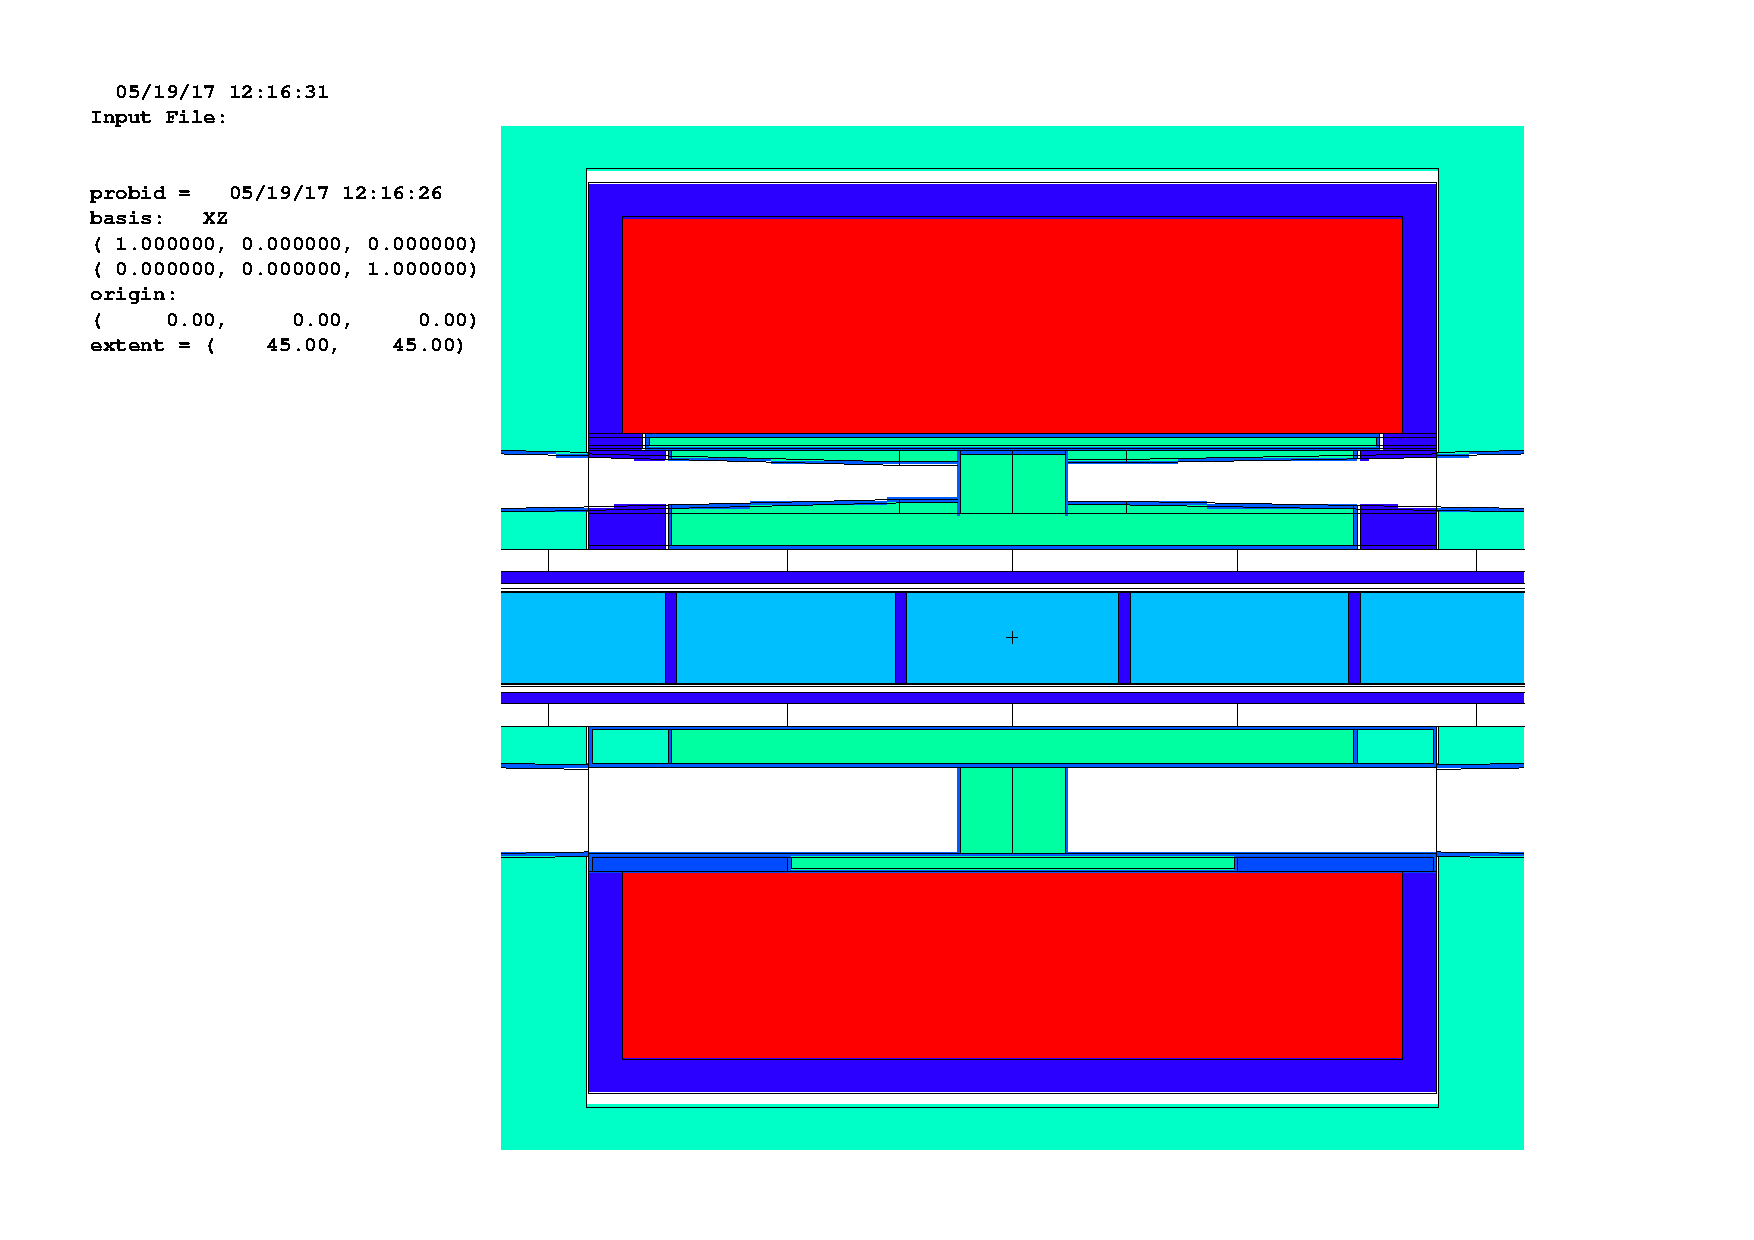
\includegraphics[width=0.5\textwidth, clip=true, trim=8.5cm 10cm 4cm 2.5cm]{UserGuide/BeRefRadius343.pdf}}~
  \subfloat[{\tt BeRefRadius} increased to \SI{40}{\centi\meter} without taking into account dependent variables, which produced geometric errors \label{fig:user:BeRef:40:wrong}]{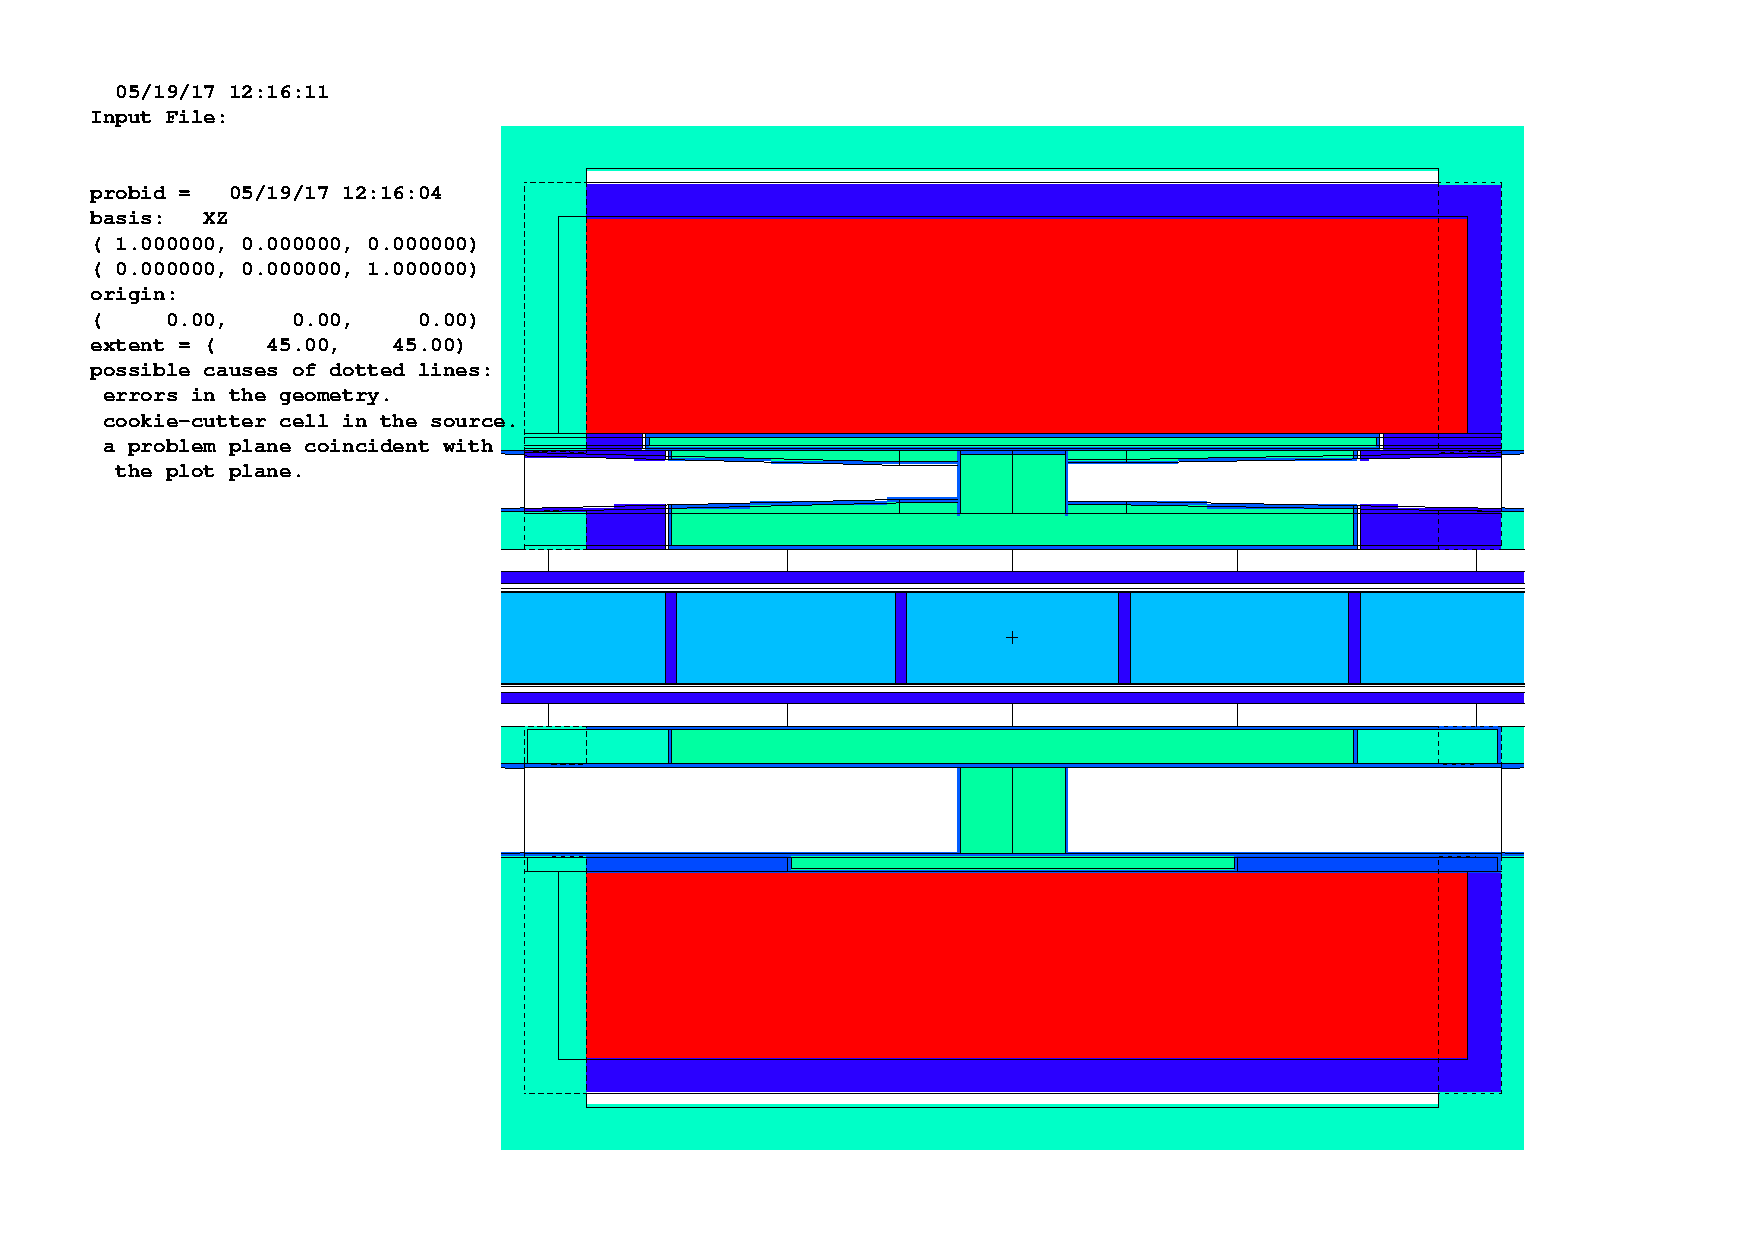
\includegraphics[width=0.5\textwidth, clip=true, trim=8.5cm 10cm 4cm 2.5cm]{UserGuide/BeRefRadius40wrong.pdf}} \\
  \subfloat[{\tt BeRefRadius} increased to \SI{40}{\centi\meter} taking into account dependent variables \label{fig:user:BeRef:40:correct}]{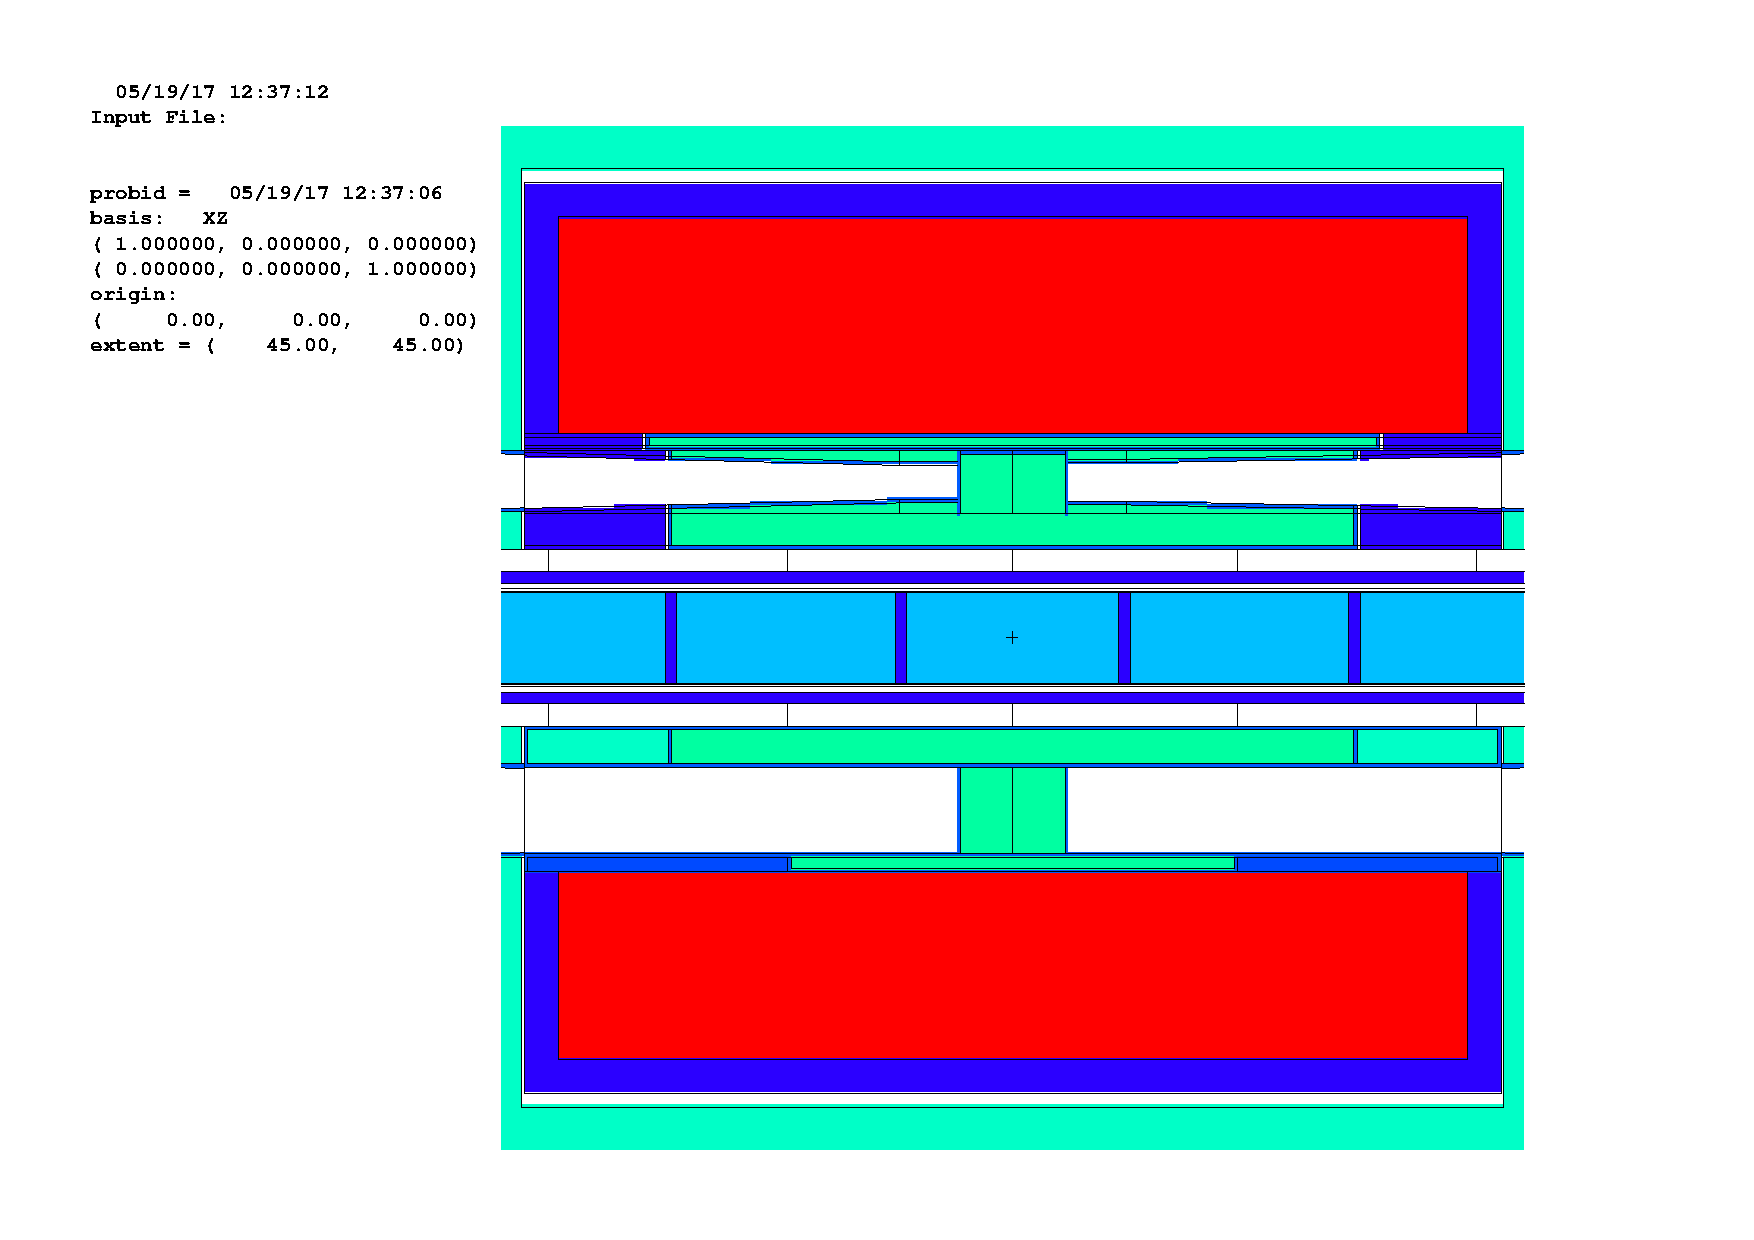
\includegraphics[width=0.5\textwidth, clip=true, trim=8.5cm 10cm 4cm 2.5cm]{UserGuide/BeRefRadius40correct.pdf}}
  \caption{Geometries with different BeRef radii}
  \label{fig:user:BeRef}
\end{figure}

In order to find out which other variables depend on the given one ({\tt BeRefRadius} in our case), find it in the variables setup in the C++ variable definition:

\begin{bash}
 grep BeRefRadius Model/essBuild/*.cxx
 Model/essBuild/essVariables.cxx:  Control.addVariable("BeRefRadius",34.3);
 Model/essBuild/essVariables.cxx:  Control.addParse<double>("BulkRadius1",
                                                   "BeRefRadius+BeRefWallThick+0.2");
\end{bash}
It means that we have to adjust the {\tt BulkRadius1} variable accordingly. This variable depends upon both {\tt BeRefRadius} and {\tt BeRefWallThick}.
Find out the {\tt BeRefWallThick} value:
\begin{bash}
  grep BeRefWallThick modelOut1.x
  c BeRefWallThick 3
\end{bash}
Therefore the {\tt BulkRadius1} value must be $40+3+0.2=43.2$\,cm:
\begin{bash}
 ./ess -r -v BeRefRadius 40 -v BulkRadius1 43.2 modelOut
\end{bash}
which produces the correct geometry shown in \figref{fig:user:BeRef:40:correct}.

\subparagraph{Important note} Sometimes in the C++ variable definitions the dependence is not set explicitly, i.e. in our case {\tt BulkRadius1} would be defined just by the value:
\begin{bash}
 Model/essBuild/essVariables.cxx:  Control.addParse<double>("BulkRadius1",43.2);
\end{bash}
In this case we have to inspect the geometry manually in order to find out which other variables we need to change to produce the correct input deck.
